\documentclass[border=10pt]{standalone}

\usepackage{tikz}
\usepackage{tikzsymbols}
\usetikzlibrary{calc,patterns,shapes.geometric}

\def\centerarc[#1](#2)(#3:#4:#5){\draw[#1] ($(#2)+({#5*cos(#3)},{#5*sin(#3)})$) arc (#3:#4:#5);}

\begin{document}
	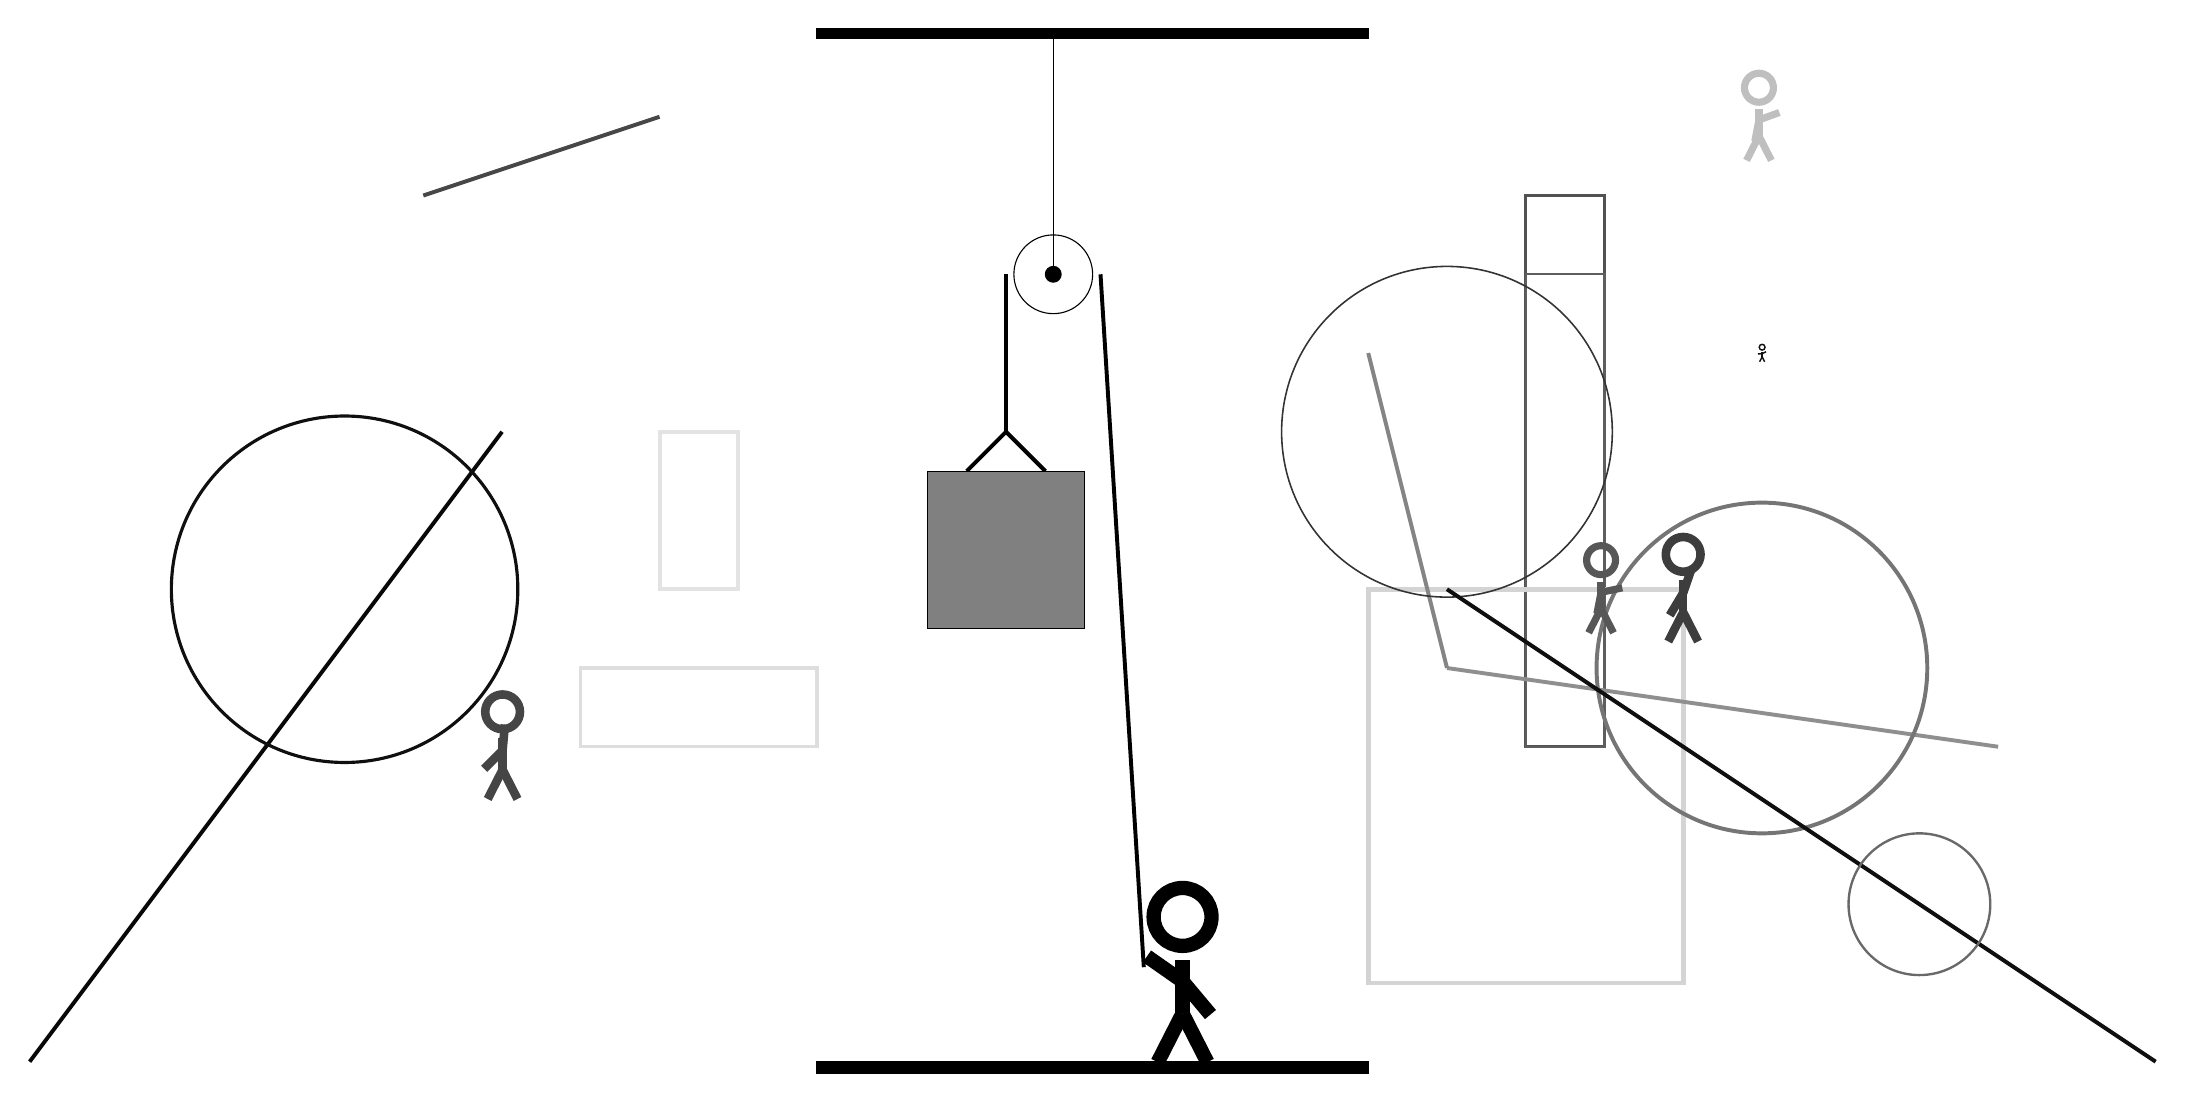
\begin{tikzpicture}
		%%%%% START %%%%%
		
		\draw[fill=black] (-2, 10) rectangle (5, 10.125);
		
		\draw (1, 7) circle (0.5);
		\draw[fill=black] (1, 7) circle (0.1);
		\draw (1, 10) -- (1, 7);
		
		\draw[line width=0.5mm] (-0.1, 4.5) -- (0.4, 5.0) -- (0.9, 4.5);
		\draw[fill=black!50] (-0.6, 4.5) rectangle (1.4, 2.5);
		
		\draw[line width=0.5mm] (0.4, 7) -- (0.4, 5.0);
		\centerarc[line width=0.5mm](1, 7)(0:180:0.6);
		\draw[line width=0.5mm](1.6, 7) -- (2.15, -1.8);
		
		\draw[line width=0.4mm, color=black!68] (7, 1) rectangle (8, 8);
		
		\draw[line width=0.3mm, color=black!63] (7, 1) rectangle (8, 7);
		\draw[line width=0.5mm, color=black!97](-6, 5) -- (-12, -3);
		\draw[line width=0.6mm, color=black!17] (5, 3) rectangle (9, -2);
		\draw[line width=0.5mm, color=black!72](-4, 9) -- (-7, 8);
		\draw[line width=0.5mm, color=black!44](6, 2) -- (13, 1);
		\draw[line width=0.5mm, color=black!48](6, 2) -- (5, 6);
		\draw [line width=0.2mm, color=black!80](6, 5) circle (2.1);
		\draw[line width=0.4mm, color=black!13] (-2, 1) rectangle (-5, 2);
		\draw [line width=0.5mm, color=black!54](10, 2) circle (2.1);
		
		\draw[line width=0.5mm, color=black!94](6, 3) -- (15, -3);
		\node[line width=0.4mm, color=black!25] at (10, 9) {\Strichmaxerl[5][79][20]};
		\draw [line width=0.3mm, color=black!59](12, -1) circle (0.9);
		
		\draw[line width=0.5mm, color=black!11] (-3, 5) rectangle (-4, 3);
		\node[line width=0.7mm, color=black!94] at (10, 6) {\Strichmaxerl[1][4][26]};
		\node[line width=0.7mm, color=black!76] at (9, 3) {\Strichmaxerl[6][59][71]};
		\draw [line width=0.4mm, color=black!94](-8, 3) circle (2.2);
		\node[line width=0.6mm, color=black!73] at (-6, 1) {\Strichmaxerl[6][45][85]};
		\node[line width=0.6mm, color=black!66] at (8, 3) {\Strichmaxerl[5][79][12]};
		
		\node at (2.6, -1.9) {\Strichmaxerl[10][-35][-50]};
		
		\draw[fill=black] (-2, -3) rectangle (5, -3.15);
		
		%%%%% END %%%%%
	\end{tikzpicture}
\end{document}